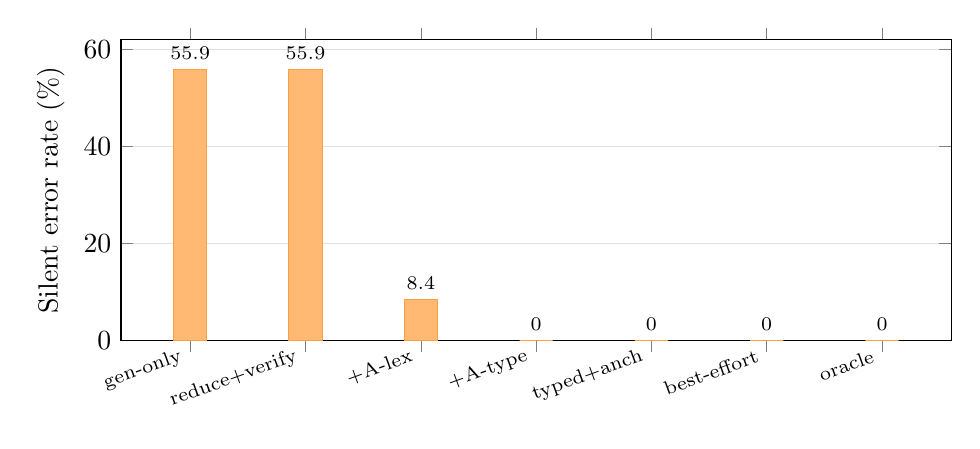
\begin{tikzpicture}
\begin{axis}[
  ybar, bar width=12pt, width=\linewidth, height=5.4cm,
  ylabel={Silent error rate (\%)}, ymin=0, ymax=62,
  symbolic x coords={gen-only,reduce+verify,+A-lex,+A-type,typed+anch,best-effort,oracle},
  xtick=data, x tick label style={rotate=20, anchor=east, font=\scriptsize},
  enlarge x limits=0.10, ymajorgrids, grid style={draw=black!12},
  nodes near coords, nodes near coords style={font=\scriptsize},
]
\addplot[fill=orange!55, draw=orange!75] coordinates {(gen-only,55.9) (reduce+verify,55.9) (+A-lex,8.4) (+A-type,0.0) (typed+anch,0.0) (best-effort,0.0) (oracle,0.0)};
\end{axis}
\end{tikzpicture}
